\documentclass[letterpaper,10pt]{article}
\usepackage{fullpage}
\usepackage{textcomp}
\usepackage{times}
\usepackage{cite}
\usepackage{fancyvrb}
\usepackage{moreverb}
\usepackage{graphicx}
\usepackage{hyperref}
\usepackage{multicol}

\makeatletter
\newenvironment{tablehere}
{\def\@captype{table}}
{}
\newenvironment{figurehere}
{\def\@captype{figure}}
{}
\makeatother

\newcommand{\squishlist}{\begin{list}{$\bullet$}
  {\setlength{\itemsep}{0pt}
    \setlength{\parsep}{3pt}
    \setlength{\topsep}{3pt}
    \setlength{\partopsep}{0pt}
    \setlength{\leftmargin}{1.5em}
    \setlength{\labelwidth}{1em}
    \setlength{\labelsep}{0.5em}
  } }

\newcommand{\squishend}{\end{list}}

\title{Freeing CUDA}
\author{Nick Black\\
Project Proposal, CS4803DGC Spring 2010}
\date{}

\begin{document}
\maketitle

\begin{abstract}
For several years, the \texttt{nouveau} project (\url{http://nouveau.freedesktop.org/wiki/})
has heroically assembled an Open Source, cleanroom implementation of 2D drivers for
NVIDIA cards\cite{nouveaustatus}. Early in 2010, RedHat Fedora Linux began driving
NVIDIA devices with \texttt{nouveau}. Shortly thereafter, NVIDIA dropped
support for their (feature-limited, shrouded-source) \texttt{nv} X.Org driver\footnote{The
closed-source \texttt{nvidia} driver is still actively supported.}. \texttt{nouveau} represents
the clear and inevitable future of NVIDIA support on the Linux/X.Org platform.

The Nouveau Project's primary aim is to provide a high-quality rendering
solution to the Linux desktop. Support for GPGPU has not been a priority, but
the path to open source GPGPU undoubtedly lies through
\texttt{Nouveau}'s advanced memory management infrastructure and well-designed hardware
abstractions, especially if it is to coexist with hardware-accelerated desktops.
As a believer in both the practical and ethical value of Open Source, I believe
it high time Linux's GPGPU stack was Freed, and that replacing \texttt{libcuda.so}
is the most immediately critical task.
\end{abstract}

\begin{multicols}{2}
\section{Project objectives}
The object of the project is to produce a practical, efficient, distributable
CUDA middleware making use of the \texttt{nouveau} driver. This will involve,
at minimum, a blackbox-equivalent source implementation of \texttt{libcuda.so}.
Modifications to the \texttt{nouveau} driver itself will almost certainly also
be required; any such modifications will require approval of the Nouveau Project.
Changes to the driver must, therefore, not compromise Nouveau's primary goal of
robust 2D performance on the Linux desktop. In this phase, it is essential that
the documented CUDA API be reproduced faithfully; existing CUDA applications can
then be harnessed to verify implementation correctness and efficiency.

Toolchain and runtime dependencies should be a subset (that is, strictly less
restrictive) than those of the \texttt{nouveau} driver itself. The library
ought be implemented, ala \texttt{libdrm\_XXX}, with an eye towards being bundled
with the driver itself (a distinct Linux kernel module is neither necessary nor
desirable). At a minimum, an API/ABI version dependency will exist between
\texttt{nouveau} and our userspace.

This project does not seek to replace the CUDA Runtime API, a set of helper
functions and subsystems designed to simplify CUDA programming. This API ought
be implementable atop our CUDA ``Driver API'' library's support, though the
existing NVIDIA \texttt{libcudart.so} is unfortunately closed source. Any
application making correct use of the Driver API ought perform equivalently atop
our infrastructure. Note that it is possible to compile \texttt{.cu} files down
to C source and Driver API calls via the \texttt{--cuda} flag to \texttt{nvcc}\cite{nvcc}.
\section{Tools}
I've interposed numerous functions to perform context-sensitive
reverse-engineering. Below is an example of \texttt{iocular}, a tool to track
changes in the memory regions passed to \texttt{ioctl}.

\begin{figurehere}
\centering
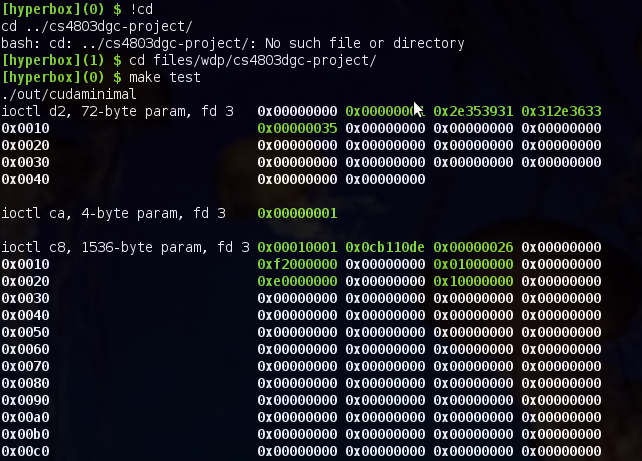
\includegraphics[width=\columnwidth]{texobjs/iocular.png}
\caption{The \texttt{iocular} tool}
\end{figurehere}
Further use has then been made of:
\squishlist
\item \texttt{vbtracetool}\cite{vbtrace} to dump video BIOS,
\item \texttt{cuda-gdb}\cite{cudagdb} to debug CUDA programs,
\item \texttt{strace}\cite{stracecode} to track system calls,
\item \texttt{nv50dis}\cite{nv50dis} to disassemble nv50 binaries,
\item \texttt{nvtrace}\cite{nvtrace} to decipher \texttt{ioctl}s issued to the NVIDIA proprietary driver, and
\item the Linux kernel's MMIOTrace\cite{mmiotrace} infrastructure to track memory-mapped I/O operations.
\squishend
\section{Methodology}
Initially, I proceeded via high-level analysis, using \texttt{strace} and
\texttt{iocular} to monitor \texttt{ioctl}s. I collected a database of ioctls
issued, the device node(s) and CUDA function(s) with which they were associated,
parameter lengths and sample inputs/outputs. I then implemented \texttt{cuInit}
based off these ioctls. Subsequent functions failed, however, and it became
clear that other elements were at work. Examining the \texttt{strace} output
more closely, it became clear that a great deal of memory-mapped I/O was at
work.

\begin{figurehere}
\centering
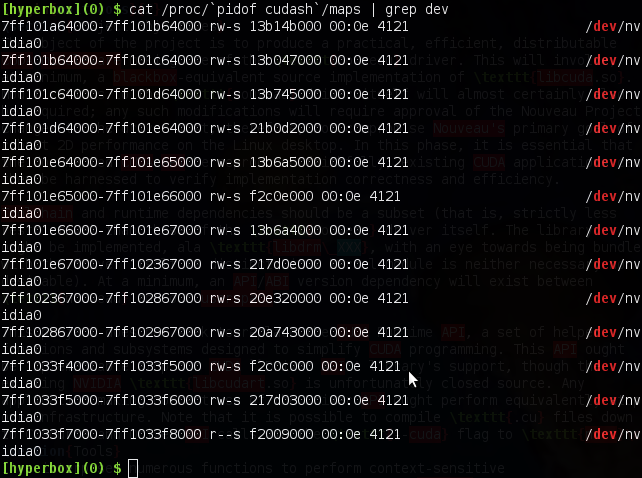
\includegraphics[width=\columnwidth]{texobjs/cudashmaps.png}
\caption{Device mappings of a sample CUDA process}
\end{figurehere}
\section{Related work}
Albert Exojo's master's thesis implemented \texttt{libecuda}\cite{exojo}, a replacement for
the CUDA Runtime API library mentioned above. The Ocelot\cite{ocelot} binary translation
framework for PTX similarly replaces the Runtime API. The former replaces the NVIDIA
hardware with an emulator; the latter recompiles PTX for NVIDIA and x86.
\bibliographystyle{acm}
\bibliography{cs4803dgcfinal}
\end{multicols}
\end{document}
